\documentclass[10pt,a4paper]{article}
\usepackage[utf8]{inputenc}
\usepackage[czech]{babel}
\usepackage[T1]{fontenc}
\usepackage{amsmath}
\usepackage{amsfonts}
\usepackage{graphicx}
\usepackage{amssymb}
\usepackage{hyperref}
\usepackage{float}
\author{David Andrešič}
\title{Programování paralelních aplikací}
\begin{document}

\begin{titlepage}
%\maketitle

\begin{minipage}{0.4\textwidth}
\begin{flushleft}
VŠB-TUO
\end{flushleft}
\end{minipage}
\begin{minipage}{0.4\textwidth}
\begin{flushright}
Datum: \today
\end{flushright}
\end{minipage}\\[5.0cm]

%\vfill

%\HRule \\[0.4cm]
\begin{center}

{\huge \bfseries Programování paralelních aplikací}\\[1.0cm]
{\huge Projekt}\\[1.5cm]
{\large Aplikace konvoluční matice na obraz}\\[4cm]

\end{center}

%\begin{tabular}{c|l}
%	{\bf Příklad} & {\bf Poznámky} \\
	
%	\hline\\[0.2cm]
	
%	1 &  \\[1.5cm]
%	2 &  \\[1.5cm]
%\end{tabular}

\vfill

\begin{minipage}{0.4\textwidth}
\begin{flushleft}
\begin{tabular}{lp{9cm}}
Vypracoval:&	David Andrešič	\\
\end{tabular}
\end{flushleft}
\end{minipage}

\end{titlepage}
%\fontsize{3mm}{3mm}\selectfont
\tableofcontents

\section{Motivace}

Aplikace tzv. konvoluční matice patří mezi základní principy v oblasti počítačové grafiky a digitálního zpracování obrazu obecně. S využitím tohoto postupu je totiž možné na digitální obraz aplikovat celou škálu filtrů od rozmazání či zaostřování, přes různé formy detekce hran či jejich vylepšení až po reliéfy.

S rozmachem paralelizace v posledních letech je zároveň možné zásadním způsobem urychlit aplikaci těchto filtrů na obraz. Digitální obraz je totiž reprezentován jako matice obrazových bodů (pixelů) a konvoluční matice je z principu aplikována tak, že nemanipuluje s body původního obrazu, ale vytváří obraz nový. Tato "disjunktnost" umožňuje jednotlivé body nového obrazu počítat paralelně dle principu SIMD (Single Instruction, Multiple Data).

V této práci jsem se tedy zaměřil na srovnání rychlosti mezi klasickou "sériovou" aplikací konvoluční matice a její paralelní obdobou realizovanou s využitím OpenCL na GPGPU.

\section{Konvoluce trochu teoreticky}

Jak již bylo zmíněno, aplikací konvoluční matice na obraz získáme nový obraz, nějakým způsobem podobný tomu původnímu. Z matematického hlediska jde o operaci dvou funkcí (původní funkce a tzv. jádra - kernelu), jejímž výsledkem je nová funkce vycházející z funkce původní (\cite{comtel}). Celou operaci lze (pro diskrétní doménu) zapsat takto:

\label{conv_eq}
\begin{equation}
(f*h)(m,n)=\sum^{M-1}_{r=0}\sum^{M-1}_{s=0}f(r,s)h(m-r,n-s)
\end{equation}

kde $f(m,n)$ a $h(m,n)$ jsou funkce z obrazového prostoru $\Omega=\{(m,n)|m=0,1,...M-1;n=0,1,...N-1\}$ (\cite{dzo}).

Lépe si však lze celou operaci představit takto:

\begin{figure}[H]
\centering
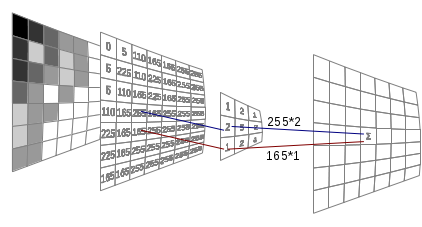
\includegraphics[scale=1.0]{images/convolution.png}
\caption{Princip aplikace konvoluční matice. Zleva: původní obraz, jeho jasová matice, na ní aplikovaná konvoluční matice, nový pixel ve výsledném obrazu. Zdroj: \cite{comtel}} 
\label{convolution}
\end{figure}

Na obrázku \ref{convolution} zcela vlevo vidíme původní obraz, který je dále převeden do formy jasové matice. V ní je na bod (4,4) aplikována konvoluční matice a výsledek této operace je ulože na pozici (4,4) v nové matici. Princip výpočtu pro prvek (4,4) je tedy následující: $(165*1)+(225*2)+(165*1)+(255*2)+(165*5)+(255*2)+(165*1)+(255*2)+(255*1)$. Tato suma se uloží na pozici (4,4) ve výsledném obrázku.

\section{State of the art}

Jelikož je konvoluční matice a její aplikace jedním ze základních prvků digitálního zpracování obrazu, setkáme se s ní v nějaké podobě téměř v každém softwaru z této oblasti. Namátkou můžeme jmenovat např. grafické editory Gimp, nebo Adobe Photoshop, kde je tento princip "schován" za celou řadou filtrů, popř. je možné si uživatelsky definovat matici vlastní. V případě Photoshopu je možné (se správnou softwarovou a hardwarovou výbavou) realizovat část jeho efektů využívající konvoluci akcelerovaně pomocí GPGPU (CUDA). Obdobnou možnost nabízí celkem čerstvě také Gimp (OpenCL). Oba nástroje slibují téměř instantní výsledky daných operací, což svým způsobem v tomto projektu ověříme.

\subsection{Algoritmy řešení}

Ačkoliv existuje i několik poměrně "exotických" algoritmů, jako např FFT konvoluce přenášející problém z prostorové oblasti na násobení ve frekvenční oblasti (vhodné zejména pro velké matice konvolučních jader - viz \cite{dzo2}), zaměříme se v tomto projektu na základní, "naivní" algoritmus vyplývající z definice aplikace konvoluční matice. Důvodem je především jeho snadná paralelizace (resp. obdobná implementace jak v sériové, tak paralelní obdobě). Výsledkem tedy je, že rozdíl mezi sériovým a paralelním řešením bude dát čistě "technologicky" a bude jen minimálně ovlivněn zvoleným algoritmem.

Z definice tedy plyne, že použijeme dva vnořené \verb|for| cykly. První bude iterovat nad všemi body jasové matice vstupního obrazu, druhý pak použije aktuální pixel v rámci dané iterace a bude iterovat nad všemi prvky konvoluční matice, přičemž bude provádět výpočet sumy dle \ref{conv_eq}. Po doběhnutí této druhé (vnitřní iterace) je výsledek sumy uložen do výsledného obrazu na stejnou pozici, jako aktuální pixel v rámci dané (vnější) iterace.

Paralelizaci tohoto algoritmu lze provést tak, že vnější \verb|for| cyklus nahradíme OpenCL \textit{kernelem} (ten tak bude obsahovat pouze vnitřní \verb|for| smyčku a potřebné reference a indexy). V rámci každé \textit{work item} ("instance" kernelu) tedy proběhne pouze vnitřní iterace nad (relativně malou) konvoluční maticí, jejíž výsledek se přímo zapíše do výsledného obrazu. 

Díky tomu, že původní obraz je ponechán beze změn (výsledky konvoluce jsou ukládány do zcela nového obrazu), může celá aplikace matice při dostatečném počtu \textit{processing units} ($>=$(počet pixelů v obrazu)) dané \textit{compute unit} proběhnout i "najednou" (to se sice týká pouze malých obrazů s řádově stovkami pixelů, i tak jsou ale za stejnou jednotku času, jako v případě sériového algoritmu, zpracovány desítky až stovky pixelů navíc).

\section{Popis implementace}

Aplikace je napsána v Javě 1.7 s využitím nativních knihoven OpenCV pro práci s obrazem a OpenCL pro realizaci paralelního algoritmu. Rozhraní je pouze textové.

\subsection{Systémové požadavky}

Pro sestavení aplikace bude potřeba následující:

	\begin{itemize}
		\item x86/x86\_64 CPU (aplikace využívá nativní knihovnu OpenCV)
		\item OS Linux/Windows
		\item Git
		\item Java Development Kit 1.7
		\item Maven >=2
		\item pdflatex pro případne sestavení doprovodného dokumentu
	\end{itemize}

	Hotový build by si měl z výše zmíněné množiny vystačit pouze s OS a Java Runtime Environment 1.7.

\subsection{Sestavení spustitelného balíku}
    
	Pomocí \textit{Maven}:
	
    \begin{verbatim}
	# pripadny presun do slozky projektu
	/lokalni/adresar/$ cd ConvolutionTool
    
	# sestaveni dokumentace (javadocs) - generuje do adresare "target/site/apidocs"
	/lokalni/adresar/ConvolutionTool$ mvn javadoc:javadoc 
	
	# sestaveni spustitelneho baliku - "uber-ConvolutionTool-1.0-SNAPSHOT.jar"
	/lokalni/adresar/ConvolutionTool$ mvn package 
	\end{verbatim}    
    
	Sestavení doprovodného dokumentu pomocí \textit{pdflatex}:
	
	\begin{verbatim}
	/lokalni/adresar/ConvolutionTool$ cd doc # presun do slozky s dokumentaci
	
	/lokalni/adresar/ConvolutionTool/doc$ pdflatex ppa_document.tex # dokument
	/lokalni/adresar/ConvolutionTool/doc$ pdflatex ppa_document.tex # znovu (cislovani)
    \end{verbatim}  
    
\subsection{Spuštění aplikace} 

Jako klasický JAR (bez parametrů vypíše nápovědu, viz příloha \ref{help}):

	\begin{verbatim}
	/lokalni/adresar/ConvolutionTool$ java -jar target/uber-ConvolutionTool-1.0-SNAPSHOT.jar
	\end{verbatim} 

\label{heap_alert}
\textbf{Upozornění:} v případě práce s velkými obrazy bude pravděpodobně nutné navýšit velikost alokovaného heapspace pro JVM:

	\begin{verbatim}
	java -Xms512m -Xmx2048m -jar target/uber-ConvolutionTool-1.0-SNAPSHOT.jar
	\end{verbatim}

\section{Experimenty}

Nadešel tedy čas porovnat obě implementace algoritmu.

\subsection{Testovací data}

Jako testovací obrázek byl použit (v oblasti digitálního zpracování obrazu velmi známý) obrázek Leny Söderberg v rozlišeních 512x512px a 2048x2048px.

\begin{figure}[H]
\centering
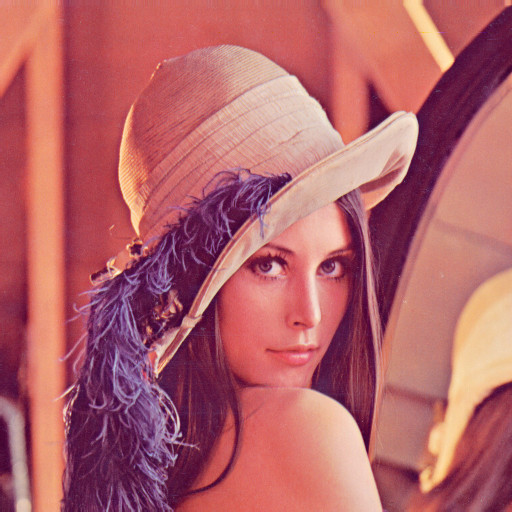
\includegraphics[scale=0.3]{images/lenna.png}
\caption{Testovací obrázek} 
\label{lenna}
\end{figure}

Na oba tyto obrázky byly aplikovány tyto konvoluční matice:

\begin{itemize}
	\item  \textit{matrix\_1=}
		\begin{math}
		\begin{bmatrix}
		  1 & 2 & 1 \\
		  2 & 4 & 2 \\
		  1 & 2 & 1 
		 \end{bmatrix}
		\end{math} 

	\item \textit{matrix\_2=}
		\begin{math}
		\begin{bmatrix}
		  0 & 1 & 0 \\
		  1 & 4 & 1 \\
		  0 & 1 & 0 
		 \end{bmatrix}
		\end{math} 
		
	\item \textit{matrix\_3=}
		\begin{math}
		\begin{bmatrix}
		  -1 & 0 & 1 \\
		  -2 & 0 & 2 \\
		  -1 & 0 & 1 
		 \end{bmatrix}
		\end{math} 
		
	\item \textit{matrix\_4=}
		\begin{math}
		\begin{bmatrix}
		  -2 & -1 & 0 & 1 & 2 \\
		  -2 & -1 & 0 & 1 & 2 \\
		  -2 & -1 & 0 & 1 & 2 \\
		  -2 & -1 & 0 & 1 & 2 \\
		  -2 & -1 & 0 & 1 & 2 
		 \end{bmatrix}
		\end{math} 
\end{itemize}

\subsection{Metodika testování}

Aplikace akceptuje na vstupu pouze jeden obrázek, byla tedy spuštěna dvakrát (jednou pro každý testovací obrázek). V rámci testovacího scénáře nejprve aplikovala výše uvedené matice pomocí sériového algoritmu a poté totéž udělala s paralelním algoritmem. Naměřené časy odpovídají pouze "pracovním smyčkám" algoritmů, tj. nikoliv přípravě dat pro aplikaci matic (v případě OpenCL jsou potřeba kroky navíc spojené s vektorizací vstupních a výstupních matic, což uměle navyšuje výsledné časy - v reálné aplikaci lze s tímto počítat a ztrátu eliminovat).

Konkrétní parametry aplikace:

\begin{verbatim}
java -Xms512m -Xmx2048m -jar target/uber-ConvolutionTool-1.0-SNAPSHOT.jar \
-i sample_data/lenna.jpg -f sample_data/matrices.xml -wl
\end{verbatim}

\subsection{Testovací sestava}

\begin{tabular}{|p{5cm}||p{7cm}|}
	
	\hline
	\textbf{Parametr} & \textbf{Hodnota}	\\
	\hline
	\hline
	CPU & Intel(R) Core(TM) i3-2328M	\\
	\hline
	Počet jader CPU (fyz./log.) & 2/4	\\
	\hline
	Frekvence CPU & 2,2GHz	\\
	\hline
	Paměť RAM & 4GB	\\
	\hline
	GPU & Intel® HD Graphics 3000	\\
	\hline
	Frekvence GPU (zákl./max.) & 650MHz/1.1GHz	\\
	\hline
	Operační systém & openSUSE 12.3 x86\_64 (GNU/Linux) \\
	\hline
\end{tabular}\\[0.3cm]

Jak je vidět, jde o poměrně běžnou sestavu s integrovanou grafickou kartou.

\subsection{Výsledky testů}

\begin{itemize}
	\item \textbf{Rozlišení 512x512px }\\[0.5cm]
	\begin{tabular}{|p{3cm}||p{3cm}|p{3.5cm}|p{2cm}|}	
		\hline
		\textbf{Matice} & \textbf{Sériový alg. [ms]} & \textbf{Paralelní alg. [ms]} & \textbf{Rozdíl [ms]}	\\
		\hline
		\hline
		matrix\_1 &					587	&						12	&							575	\\
		\hline
		matrix\_2 &					593	&						3	&							590	\\
		\hline
		matrix\_3 &					515	&						3	&							512	\\
		\hline
		matrix\_4 &					1173&						5	&							1168\\
		\hline
		\hline
		\textbf{Celkem:}	&		2868&						23	&							2845\\
		\hline
	\end{tabular}\\[0.3cm]

	Implementace pomocí OpenCL je \textbf{124,7x} rychlejší (rozdíl: 2,845s).
	
	\item \textbf{Rozlišení 2048x2048px}\\[0.5cm]
	\begin{tabular}{|p{3cm}||p{3cm}|p{3.5cm}|p{2cm}|}	
		\hline
		\textbf{Matice} & \textbf{Sériový alg. [ms]} & \textbf{Paralelní alg. [ms]} & \textbf{Rozdíl [ms]}	\\
		\hline
		\hline
		matrix\_1 &					7308	&						74	&							7234	\\
		\hline
		matrix\_2 &					7276	&						44	&							7232	\\
		\hline
		matrix\_3 &					6995	&						54	&							6941	\\
		\hline
		matrix\_4 &					17260	&						80	&							17180	\\
		\hline
		\hline
		\textbf{Celkem:}	&		38839	&						252	&							38587	\\
		\hline
	\end{tabular}\\[0.3cm]
	
	Implementace pomocí OpenCL je \textbf{154,12x} rychlejší (rozdíl: 38,587s)
	
\end{itemize}

\section{Závěr}

Předně je potřeba upozornit, že výsledky první matice počítané na OpenCL jsou zjevně mírně zkresleny režií spojenou s inicializací nativních knihoven. Toto zkreslení by se dalo dále odstranit např. "podstrčením" falešného obrázku, který by se do testovací dávky nepočítal a pouze by zajistil potřebnou inicializaci, nicméně na výsledku to příliš nemění.

Na základě experimentů lze usuzovat, že OpenCL plně demonstrovalo sílu GPGPU výpočtů, když i na průměrné sestavě s integrovanou grafikou překonalo výkon algoritmu vykonávaného sériově na CPU o mnoho více než stonásobek. Byť je potřeba dodat, že tyto výsledky obecně záleží na konkrétním problému a jeho paralelizaci (kde maticové operace patří obecně mezi dobře paralelizovatelné problémy). Výsledky zároveň poukazují na to, že s rostoucími rozměry matic se propast mezi výkonem CPU a GPU prohlubuje.

\begin{thebibliography}{9}

	\bibitem{comtel} Implementace konvoluce. [online]. [cit. 2014-01-19]. Dostupné z: www.comtel.cz/files/download.php?id=5464
	
	\bibitem{dzo} SOJKA Eduard. Matematické základy digitálního zpracování obrazu. [online]. 2011 [cit. 2014-01-19]. Dostupné z: http://mrl.cs.vsb.cz/people/sojka/dzo/mzdzo.pdf
	
	\bibitem{dzo2} FABIÁN Tomáš. Digitální zpracování obrazu - Cvičení 2. [online]. 2013 [cit. 2014-01-19]. Dostupné z: http://mrl.cs.vsb.cz/people/fabian/dzo/konvoluce.pdf
	
\end{thebibliography}

\appendix 
\section{Kompletní nápověda aplikace}
\label{help}

\begin{verbatim}
usage: uber-ConvolutionTool-1.0-SNAPSHOT.jar
 -d,--debug                         enables the debug mode (maximal
                                    verbosity)
 -f,--matrix-file <arg>             path to the XML containing the
                                    convolution matrices
 -h,--human-readable                enables the human readable time output
 -i,--input-image <arg>             the input image's filaname
 -l,--log <arg>                     enables the logging to a file
 -si,--show-input-image             show input image when loaded
 -so,--show-output-image            show input image(s) when loaded
 -wl,--measure-working-loops-only   measures only the working loops


\end{verbatim}

\section{Struktura XML s konvolučními maticemi}
\label{xml}

\begin{verbatim}
<?xml version="1.0"?>
<matrices>
    <matrix name="matrix_1">
        <row>
            <col>1</col>
            <col>2</col>
            <col>1</col>
        </row>
        <row>
            <col>2</col>
            <col>4</col>
            <col>2</col>
        </row>
        <row>
            <col>1</col>
            <col>2</col>
            <col>1</col>
        </row>
    </matrix>

    <matrix name="matrix_2">
        <row>
            <col>0</col>
            <col>1</col>
            <col>0</col>
        </row>
        <row>
            <col>1</col>
            <col>4</col>
            <col>1</col>
        </row>
        <row>
            <col>0</col>
            <col>1</col>
            <col>0</col>
        </row>
    </matrix>
</matrices>

\end{verbatim}

\end{document}